\chapter{Design and Architecture}
\section{Design}
The design of software application needs a well defined problem, when a new improved design of a user interface is needed. Main focus lays in easy navigation, responsive interface and intuitive access to the most needed parts of the system. \todo{rewrite introduciont to chapter}.

\subsection{The focus}
The focus of new design lays in improving the user experience. This application is integrateing GitHub for safe login system, access to git repositories through authentication, and gives the user easy controll over the repositories relevant to specific courses. The system is designed is such a way so that both students and teachers have intuitive access to the parts of the system that they use most frequently. There exists student section and teacher section, these are called "modes"\worry{insert something about admin mode?}, having Autograder in teacher mode, one can easily create a new course and rename it, GitHub integration \ref{gihubintegration} takes care of creating and managing the repositories needed in that course, initial setup of a course is done through a course setup page. The management of students that have joined the course, involves actions like creating group assignments, expelling students and approving new studends who joined the course, these can be done in the course management page. Most used functionality, by both teachers and teaching assistants is course lab overview. This lets a teacher quickly skim through all the students and look if anyone hasn't delivered their assignment yet, or see the score of each assignment, from there, it is also possible to approve or reject any given lab assignment. Another function is to be able to easily controll group assignments, and assign students to specific groups. In the group management page, there exists a user friendly interface for creating new groups and adding available students to any given group, users can be notyfied about which group they have been assigned to, similarly, students can easily create groups that need to be approved by the teachers. Students will utilize Autograder manilny for checking if their assignment has been approved. The default page for in student mode would be lab overview, there one can see the current assignment and its progress, the default course is the one choosen on last session when the user was logged in, it is also worth mentioning that usually one student wont be using Autograder in more than one course, but the system is designed for easy switch between different courses. Another userbase for Autograder are teaching assistants, they are both users and teacher in other courses, this is where Autograder modes come in handy, while working as a TA, user can switch to teacher mode and has access to the teaches functionality in the courses he teaches, similarly switching to student mode gives quick access to relevat functions in taht mode.
\subsection{Planning of software solutions}
To achieve the goal of better, quicker and more responsive interface, the front-end application is written in JavaScript. By using new emerging open source technologies and libraries like React.js, new possibilities were open. In Model View Controller (more about it in section \ref{sec:mvc}) React would stand for View, that is what user sees, and interacts with. What is missing is something to controll the user interface and the datastructures that it displays. This is achieved by structuring the application with one of many software architectures that are available. Altered way of doing things was introduced with Flux architecture, the way to write gode in flux is to isolate every UI component and send every updated piece of thata through a central hub that will dispach it further, and other components can be set up to listen to those specific changes they are interested in, more about Flux in section \ref{sec:flux}.
\\
\todo{}
\subsection{User stories}
User stories are a way to describe what application does, and what it is supposed to do in easy to read short sentences. The focus here is to give a good fundament of what the applications is being developed for. Since there is a lot of functionality to be implementet, with the help of user stories is is possible to concentrate on one functionality described by that user story at a time. One example of a user storie would be \emph{"As a teacher I want to be able to easily create groups for assignments, so that i don't have to approve student created groups."} fig: \ref{fig:groupmanagement}, \worry{choose better user story maby?} this describes vaguely what a certain user would like to do with the application, by looking at this user story, a set of tasks is being created, if there are parts of the system that need to be thought out again, or what new implementations are needed to be in place before this functionality can be implemented. With each new user story, the complexity of the application grows, and user interface should be theoretically improving on each cycle due to the way in which new functionality is implemented, since the flow of the application is being thought out and some initial design flaws might be discovered, things need to be either redesigned or a new solution found before this new functionality can be implemented. \todo{More}

\subsection{Wireframes}
Creating wireframes is a crucial part of user interface design. The point of wireframes is to have something that is easier to change than the code to be developed. Before coming to the programming phase, one can iterate over a lot more design propositions, and is able to change things up easily during this initial or planning phase. Wireframes are foundation of the application being developed, they are not supposed to show the creative design, but rather reflect on the technological and use-related aspects of the application. Before the development of new user story takes action, sketches and drawings of user interface are being produced. This is done to eliminate flaws in the interface design before they are implemented, a couple of iterations of drawing are done and evalueted from the users perspective. When this initial phase is done, more sophisticated drawings or wireframes are being created. These more detailed drawings with descriptions of areas of the interface, describe what certain elements of this user interface do. Serving as a blue print for further developing of the interface.
\begin{figure}[h]
  {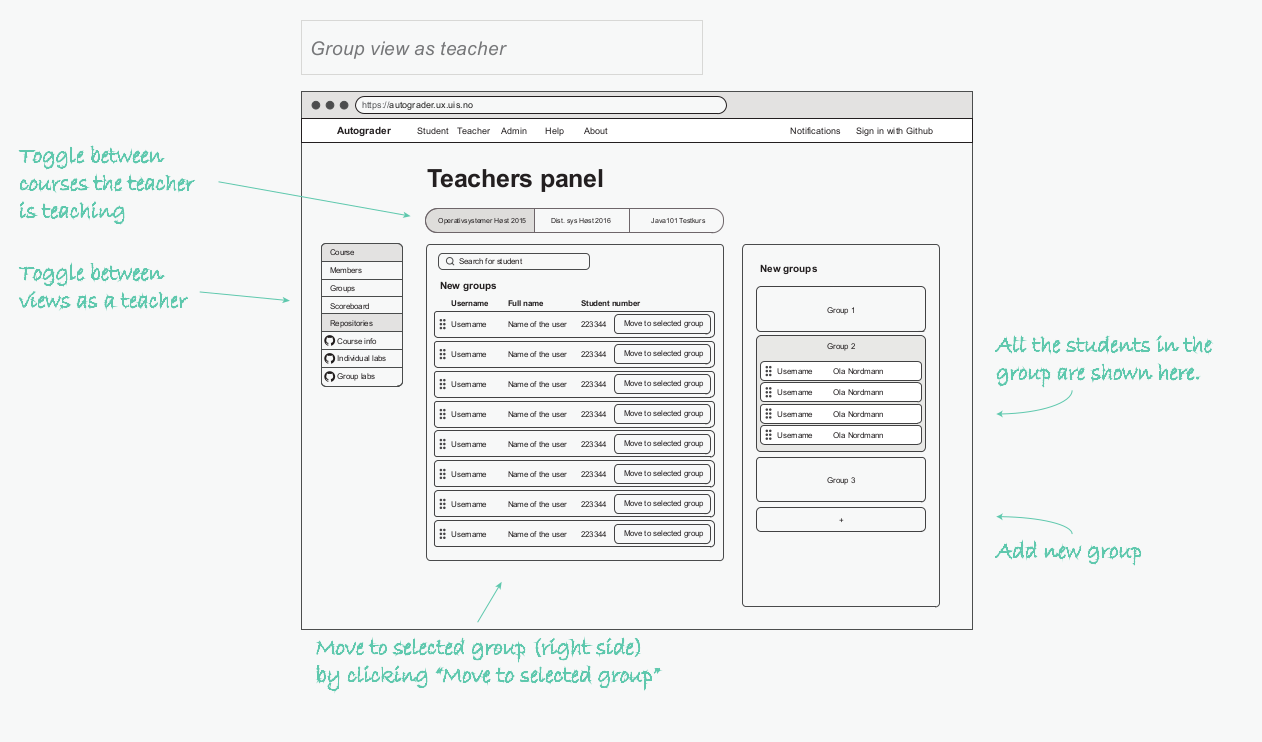
\includegraphics[width=1\linewidth]{groupmanagement}}
  \caption{Wireframes for Group management page}
  \label{fig:groupmanagement}
\end{figure}
\\Wireframe figure above was created as a result of a user story, next step is to create reflection of that wireframe in code, 


\section{Development process}
\worry{not sure about this section, is it usefoul for the reader?}\\
What enables us to finish the design as it was planned is good workflow, this is there are a couple of ways to go about it, they improve the effectivity and productivity of the process of developing new software solution.
\subsection{Kanban / Scrum}
\todo{explain short kanban and scrum}

\section{Architecture}
Architecture of the Autograder system describes the high level structures developed while working on the application. Choice of software architecture, software models on both front and back-end are things that are crucial aspects of creating good application.
\subsection{Software architecture}
Autograder is an application for teachers and students, the new version is going to be running on local university network and is going to be accessible from anywhere on the internet, that means there is no restrictions as to what network you are trying to access it from. Primary use for teachers is creating courses in the Autograder system that are associated with the courses at the university, each course has a GitHub repository associated with it, and configured to the needs of that course. This means that an implementation of GitHub integration needs to be created, this is mainly the focus of back-end part of the software, still the front-end, or web client, needs to be designed in such a way to enable the use such integration. The client is not supposed to serve as an alternative view of GitHub repositories, GitHub is mainly used as a place to easily store source code, and its authentication system. The client needs to be able to display courses that a student is enrolled into, assignments that the teacher has published to that course, that also involves group assignments.
\\Although the data is stored in the databse, manipulation of that data is done on the client side, and then sent further to the back-end for interpretation and updating the storage. Similarly it is also possible to update the client from the back-end, either directly or through the actions of another client. The user interface updates in real time, as an example, lets take a teacher that is assigning students to group assignmets, teacher is using an interactive interface to manipulate the users into selected groups, the student is simultaneusly notfied in real time when he gets assigned to a new group withouth the need of refreshing the page \worry{better example here}. Teachers can be notified when a new student has enrolled to course, or one of the students has exceeded his slip-days for an assignment. Real time updates are possible due to the connection protocol used in the application. When a client connects to the autogader server, client application requests for a protocol upgrade, from then on all data transfer is done through \emph{websocket prodocol}\cite{websocket}. This enables the server to push its updates to all clients, without being explicetly asked about it by them.
\\The reasoning behind real-time update system was that notifications and responsiveness of user interface was one of the primary reasons for developing this application. Although one could argue that orther methos of updating the UI and notifications would be sufficient, like polling or long-polling, that is frequent client requests for update from the server, websocket protocol has no obvoius disatvantages to the presented solution, and at the same time opens possibilities for further upgrades of the system, like chat functionality, which could be utilized for questions related to assignments.
\subsection{MVP or Model View Controller}\label{sec:mvc}

\subsection{Flux}\label{sec:flux}

\subsection{Other}

\subsection{Backend}
start
\subsubsection{Server}
\textbf{Go}
\subsubsection{Database}
\textbf{SQL}
\textbf{noSQL}
\subsection{Frontend}
start
\subsubsection{Angular}
\subsection{React}

\chapter{Design and Technology @depricated}
Planning user interface involves a lot of time spent at the drawing board, without a lot of coding. This is necessary to avoid rewriting big shank's of code over and over again. Things like wireframes, use cases and user stories are used to build fundamentals for a new user interface.

During this project a software development methodology called scrum was used, this helps manage product development process significantly. In scrum, planning phase never ends, there is a endless loop of planning and implementation as the project develops. This gives a bit more freedom while drawing wireframes, the focus is on one or two specific features of the software and iterating until the feature is finished.\\\\
\section{User stories and use cases}\label{userStoriesAndUseCases}
To achieve the goad of creating good user interface, a lot of work needs to be put in going through how the applications is going to be used in theory. We create a set of use cases, these describe individual functions that the user would want to execute. This can be shown in a form of a graph, that starts usually at the default state of the software and traverses and lists actions that are needed to achieve the goal.\\\\
User stories are supposed to help develop good use cases, they are sentences that describe The type of a user, the goal and reasoning behind a given action. An example would be:\\\emph{As a administrator, I want to get to the users section, so that I can remove a user}.\\
This gives a great starting point for creating good use case, user stories are created by comping up with the actions relevant to the purpose of the software. By looking at user stories, decision is made on which of the user stories are a priority. Next an appropriate use case is made.
\section{ReactJS}\label{technologies}
In this thesis a couple of new technologies and frameworks were used. ReactJS is a JavaScript library for building user interfaces, it abstracts away the DOM from a programmer, gives a programming model similar to OOP\footnote{Object oriented programming}  to generate appropriate html document. An additional extension of React, called react-bootstrap was used to make the creative design of the application easier. React-bootstrap is just a normal twitter bootstrap\footnote{twitter url} wrapped in syntax that reassembles that of React elements.\\\\
There are a lot of problems with the solution involving ReactJS. First of all this library is created with so called single-page applications in mind, alternatively React could be used to implement smaller portions of a website, like a real time chat window, while the rest of a page is generated in a different way.\\\\
First complication is the amount of computation that is needed for a large complicated application to be generated with React. While small application like messaging app or chat window works great with React, a bit more thought needs to go into design of much more complicated applications like Autograder. \\\\
Application that was written with React is being compiled to one JavaScript file, this is the source file of the whole front-end of the application. This means that server is serving out one file and the rest is being compiled on the client side, the necessary data is being fetched from the server as it's needed, see section \ref{websocets} on websockets.\\\\
The problem arises when deciding on what should be rendered and when. It's obvious that we do not show or render every application element at once, we need a way to split the rendering into \emph{views} in other words have multiple states of the application that are associated with given url. We can achieve that by having switch statements in out code that looks at the given url, and determines what part of the code should be evaluated and rendered. This might get complicated as the application grows, to help us manage both the url states and overall improve the code readability, another library that was build on top of React was used.\\\\
React-router is a routing library that takes care of managing urls, and helps organize routes by simply looking at the nesting patter of the UI components that you want to render, furthermore it is possible to determine the parents and child elements by looking on either url or nesting patter in code, this helps make the code more readable and is helpful when debugging.

\section{WebSocets}\label{websocets}
WebSocets is a protocol that enables two-way communication between a client that is running untrusted code, and a host that is configured to communicate from that code. With this one can send and receive event-driven responses without having to poll the server for a reply. The decision to use WebSocets was somehow indirect, while working with React, it became obvious that the old pattern for receiving data from server would not be optimal for the the way React works and the way the development of the Autograder goes.\\\\
React works by listening to the changes on separate UI components, and updating their state in real time. When fetching data asynchronously, by using techniques like AJAX, the only way to update UI component is to poll the server for change and ask React to re-render on that basis. Although this is not a bad way to do things, and Autograder does not really need a lot of polling to work correctly, there are no obvious disadvantages of using WebSocets, on top of that, the way it works is more similar to the way React does things client side.\\\\
The advantages of having constant connection to the server are that the contents on the page can be updated in real time when the server updates its state. One of the use cases that came up while discussing Autograder, was to have some sort of notification system built in the system. The problem was that in the prevois version of Autograder, it was almost impossible to tell whenever someone enrolled to a course or some other important event happend in the system that needed Admin og Teacher attention, without looking for that specific event. Despite the fact that notification systems are fully possible to implement by doing it AJAX way, it would still require an event on the client side to trigger the update and notify the user, with connection based communication the update would happend almost instantly.\\\\
As mentioned before, WebSocets integrates pretty well with React, the way to do it, just simply listen to the incoming data through the WebSocet connection, and set the components underlying state - while react listens to the componetns state, it will render when changes are detected.
\section{Bootstrap}\label{bootstrap}
\lstset{
  numbers=left,
  stepnumber=1,    
  firstnumber=1,
  numberfirstline=true
}
\begin{lstlisting}
<Button>
   <div>
     <a></a>
   </div>
</Butoon>
\end{lstlisting}
